\documentclass[11pt,a4paper]{article}
\usepackage[T1]{fontenc}
\usepackage[utf8]{inputenc}
\usepackage{lmodern}
\usepackage{textcomp}
\usepackage[left=1.8cm,right=1.8cm,top=3.0cm,bottom=2.2cm,headheight=36pt,headsep=12pt]{geometry}
\usepackage{multicol}
\usepackage{xcolor}
\usepackage{fancyhdr}\usepackage{tikz}
\usepackage{graphicx}
\usepackage{array}
\usepackage{amsmath,amssymb}
\usepackage{setspace}
\usepackage{longtable}
\graphicspath{{../}}
\definecolor{ygreen}{RGB}{46,139,87}\definecolor{dgreen}{RGB}{28,90,56}
\renewcommand{\normalsize}{\fontsize{10.9}{13.4}\selectfont}
\renewcommand{\familydefault}{\rmdefault}
\setlength{\parindent}{0pt}
\setlength{\columnsep}{0.8cm}
\setlength{\columnseprule}{0.4pt}
\setlength{\multicolsep}{3pt plus 1pt minus 1pt}
\renewcommand{\textsubscript}[1]{\ensuremath{_{\text{\fontsize{8}{8}\selectfont #1}}}}
\renewcommand{\textsuperscript}[1]{\ensuremath{^{\text{\fontsize{8}{8}\selectfont #1}}}}
\newcommand{\qn}[1]{\textbf{\fontsize{11.5}{13}\selectfont #1}}
\newcommand{\qsep}{\par\vspace{13pt}}
\newcommand{\fwrule}{\par\vspace{5pt}\noindent\rule{\linewidth}{1.4pt}\par\vspace{7pt}}
\newsavebox{\fitb}
\newcommand{\fitbox}[1]{\sbox{\fitb}{#1}\ifdim\wd\fitb>\linewidth\resizebox{\linewidth}{!}{\usebox{\fitb}}\else\usebox{\fitb}\fi}
\newcommand{\diqqat}[1]{\par\smallskip\noindent\textbf{Diqqat!} #1\par\medskip}
\newcommand{\javob}{\par\nopagebreak[4]\smallskip\noindent\textbf{Javob:} \rule[-2pt]{7.5cm}{0.4pt}\par\smallskip\noindent\textbf{Diqqat!} Javobingizni javoblar varaqasiga ko`chirib yozing.\par\medskip}
\pagestyle{fancy}
\fancyhf{}
\renewcommand{\headrulewidth}{1.6pt}\renewcommand{\headrule}{{\color{ygreen}\hrule height 1.6pt width\headwidth}}
\newcommand{\hdrlogo}{
\begin{tikzpicture}[baseline=0pt]\fill[ygreen,rounded corners=3pt] (0,0) rectangle (0.95,0.95);\node[white,font=\fontsize{24}{26}\bfseries\selectfont] at (0.475,0.47){K};\node[anchor=west,font=\fontsize{16}{18}\bfseries\selectfont,text=dgreen] at (1.15,0.66){KIMYO};\node[anchor=west,font=\footnotesize\scshape,text=gray] at (1.15,0.2){Milliy sertifikat\ \ 2026};\end{tikzpicture}}
\newcommand{\hdrpill}[1]{\begin{tikzpicture}[baseline=0pt]\node[fill=ygreen,text=white,rounded corners=8pt,inner xsep=10pt,inner ysep=5pt,font=\fontsize{13}{15}\bfseries\selectfont] at (0,0.475){#1};\end{tikzpicture}}
\fancyhead[L]{\hdrlogo}
\fancyhead[R]{\hdrpill{20-variant}}

\fancyfoot[C]{\thepage}
\fancypagestyle{first}{\fancyhf{}\renewcommand{\headrulewidth}{1.6pt}\renewcommand{\headrule}{{\color{ygreen}\hrule height 1.6pt width\headwidth}}\fancyhead[L]{\hdrlogo}\fancyhead[R]{\hdrpill{20-variant}}\fancyfoot[C]{\thepage}}
\begin{document}
\normalsize
\thispagestyle{first}
\noindent\textit{Davriy jadvaldan foydalanish mumkin.}
\par\smallskip
\begin{multicols}{2}
\noindent\qn{1.} Na\textsubscript{2}CO\textsubscript{3} eritmasida gidrolizlanish darajasini oshirish uchun qaysi usullar qo`llanadi? 1) suyultirish; 2) HCl qo`shish; 3) qattiq Na\textsubscript{2}CO\textsubscript{3} qo`shib, konsentratsiyani oshirish; 4) qizdirish

\noindent A)~\textsl{1, 2, 3} \hfill B)~\textsl{1, 3, 4} \hfill C)~\textsl{1, 2, 4} \hfill D)~\textsl{3, 4}\par
\qsep
\noindent\qn{2.} Fe\textsubscript{2}O\textsubscript{3} tarkibida temir ning \textbf{valentligini aniqlang.}

\noindent A)~\textsl{VII} \hfill B)~\textsl{III} \hfill C)~\textsl{\textit{V}} \hfill D)~\textsl{II}\par
\qsep
\noindent\qn{3.} Jadvalda bog`lar hosil qiluvchi atomlarning elektrmanfiyliklari berilgan:
\begin{center}
\renewcommand{\arraystretch}{1.15}
\fitbox{\begin{tabular}{|c|c|c|}\hline
\textbf{Bog`} & \textbf{EM (1-atom)} & \textbf{EM (2-atom)} \\ \hline
Na--Cl & 0,9 & 3 \\ \hline
Mg--O & 1,2 & 3,5 \\ \hline
H--O & 2,1 & 3,5 \\ \hline
K--Br & 0,8 & 2,8 \\ \hline
\end{tabular}}
\end{center}
Qaysi bog` eng qutbli (eng ko`p ionli xarakterga ega)?

\noindent A)~\textsl{Na--Cl} \hfill B)~\textsl{H--O} \hfill C)~\textsl{Mg--O} \hfill D)~\textsl{K--Br}\par
\qsep
\noindent\qn{4.} Kislorod (\textit{Z} = 8) atomining tashqi energetik pog`onasidagi elektronlar \textbf{sonini aniqlang.}

\noindent A)~\textsl{7} \hfill B)~\textsl{5} \hfill C)~\textsl{6} \hfill D)~\textsl{8}\par
\qsep
\noindent\qn{5.} Rasmda davriy jadvalning bir qismi berilgan (\textit{X}, \textit{Y}, \textit{Z} --- noma'lum elementlar).
\begin{center}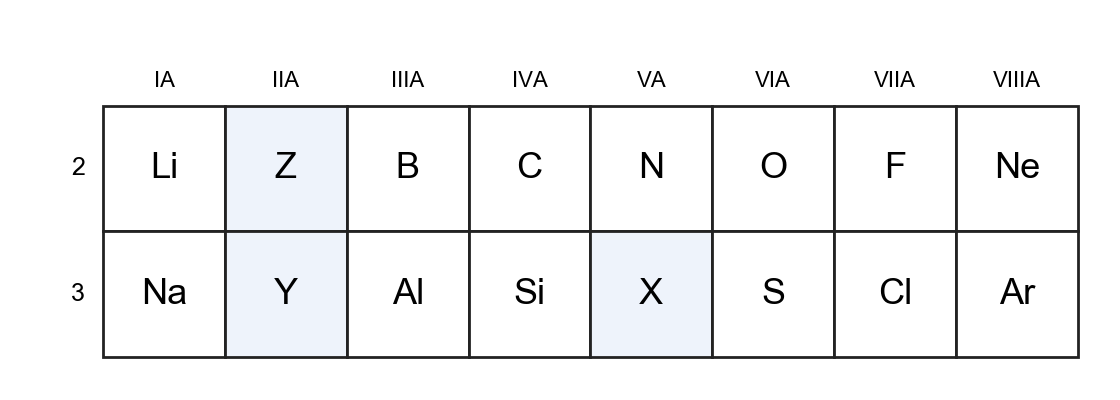
\includegraphics[width=0.86\linewidth]{rasmlar/gen/pt_229053.png}\end{center}
\textit{X}, \textit{Y}, \textit{Z} elementlardan qaysi birining atom radiusi eng katta?

\noindent\begin{tabular}{@{}p{0.47\linewidth}@{}p{0.47\linewidth}@{}}
A)~\textsl{\textit{X}} & B)~\textsl{\textit{Z}} \\
C)~\textsl{radiuslari teng} & D)~\textsl{\textit{Y}} \\
\end{tabular}\par
\qsep
\noindent\qn{6.} AgNO\textsubscript{3} ning suvli eritmasi inert elektrodlar bilan elektroliz qilinganda qaysi moddalar ajraladi?

\noindent\begin{tabular}{@{}p{0.47\linewidth}@{}p{0.47\linewidth}@{}}
A)~\textsl{Zn, H\textsubscript{2} va O\textsubscript{2}} & B)~\textsl{Ag va O\textsubscript{2}} \\
C)~\textsl{Cu va Cl\textsubscript{2}} & D)~\textsl{Cu va O\textsubscript{2}} \\
\end{tabular}\par
\qsep
\noindent\qn{7.} 4 g He 27 \textdegree{}C va 4 atm bosimda qancha hajm (l) egallaydi? (R = 0,082 l$\cdot$atm/(mol$\cdot$K))

\noindent A)~\textsl{12,3} \hfill B)~\textsl{3,08} \hfill C)~\textsl{6,15} \hfill D)~\textsl{22,4}\par
\qsep
\noindent\qn{8.} NH\textsubscript{4}Cl eritmasida gidrolizlanish darajasini oshirish uchun qaysi usullar qo`llanadi? 1) suyultirish; 2) qattiq NH\textsubscript{4}Cl qo`shib, konsentratsiyani oshirish; 3) NaOH eritmasi qo`shish; 4) qizdirish

\noindent A)~\textsl{1, 4} \hfill B)~\textsl{2, 3, 4} \hfill C)~\textsl{1, 3, 4} \hfill D)~\textsl{2, 3}\par
\qsep
\noindent\qn{9.} 0,1 mol NH\textsubscript{3} tarkibidagi atomlar \textbf{sonini toping} (N\textsubscript{A} = 6,02$\cdot$10\textsuperscript{23}). Javobni 10\textsuperscript{23} birligida yozing.

\noindent A)~\textsl{0,241} \hfill B)~\textsl{0,482} \hfill C)~\textsl{0,12} \hfill D)~\textsl{0,06}\par
\qsep
\noindent\qn{10.} Grafikda tuzning eruvchanligi (g/100 g suv) haroratga bog`liq ko`rsatilgan.
\begin{center}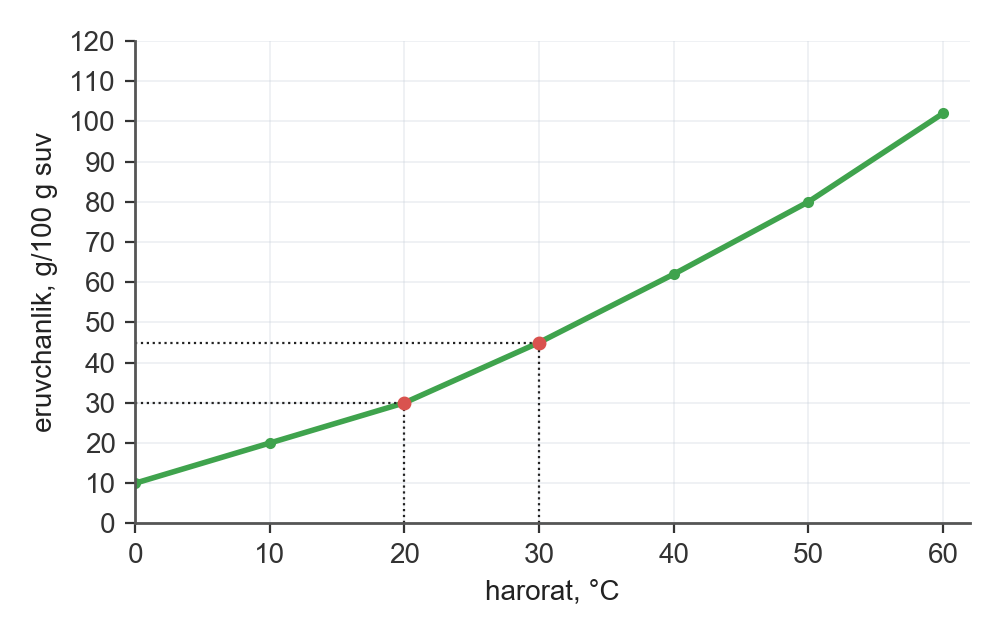
\includegraphics[width=0.86\linewidth]{rasmlar/gen/sol_v20_0.png}\end{center}
30 \textdegree{}C da tuzning to`yingan eritmasidagi massa \textbf{ulushini (\%) aniqlang.}

\noindent A)~\textsl{45} \hfill B)~\textsl{15,5} \hfill C)~\textsl{23,1} \hfill D)~\textsl{31}\par
\qsep
\noindent\qn{11.} Quyidagi jadvalda NaNO\textsubscript{3} tuzining eritmalari keltirilgan:
\begin{center}
\renewcommand{\arraystretch}{1.15}
\fitbox{\begin{tabular}{|c|c|c|}\hline
\textbf{No.} & \textbf{m(eritma), g} & \textbf{$\omega$, \%} \\ \hline
I & 200 & 5 \\ \hline
II & 300 & 35 \\ \hline
\end{tabular}}
\end{center}
Eritmalar aralashtirildi. Oxirgi eritmadagi tuzning massa \textbf{ulushini (\%) toping.}

\noindent A)~\textsl{23} \hfill B)~\textsl{20} \hfill C)~\textsl{40} \hfill D)~\textsl{17}\par
\qsep
\noindent\qn{12.} N\textsubscript{2} va O\textsubscript{2} aralashmasi tarkibida aralashmadagi protonlarning umumiy soni 9,4$\cdot$N\textsubscript{A}. Aralashmaning hajmi 13,44 l (n.sh.). Aralashmadagi N\textsubscript{2} ning \textbf{massasini (g) toping.}

\noindent A)~\textsl{2,8} \hfill B)~\textsl{16} \hfill C)~\textsl{5,6} \hfill D)~\textsl{9,4}\par
\qsep
\noindent\qn{13.} 2NO + O\textsubscript{2} $\rightleftarrows$ 2NO\textsubscript{2} reaksiyasi 5 l hajmli idishda o`tkazildi. Ma'lumotlar jadvalda berilgan:
\begin{center}
\renewcommand{\arraystretch}{1.15}
\fitbox{\begin{tabular}{|c|c|c|c|}\hline
\textbf{Modda} & \textbf{NO} & \textbf{O\textsubscript{2}} & \textbf{NO\textsubscript{2}} \\ \hline
Boshlang`ich, mol & 4 & 2 & 0 \\ \hline
Muvozanatda, mol & --- & --- & 1 \\ \hline
\end{tabular}}
\end{center}
NO ning necha foizi reaksiyaga \textbf{kirishganini aniqlang.}

\noindent A)~\textsl{12,5} \hfill B)~\textsl{37,5} \hfill C)~\textsl{25} \hfill D)~\textsl{75}\par
\qsep
\noindent\qn{14.} Ishqoriy metallar haqida qaysi fikrlar to`g`ri? 1) KOH -- kuchli ishqor; 2) Natriyning olinishi suyuqlanma NaCl elektrolizi bilan; 3) Natriy atomining tashqi qavatida 2 ta elektron bor; 4) Natriy suv bilan reaksiyada H\textsubscript{2} va NaOH hosil qiladi

\noindent A)~\textsl{2, 4} \hfill B)~\textsl{1, 2, 4} \hfill C)~\textsl{1, 2} \hfill D)~\textsl{2, 3}\par
\qsep
\noindent\qn{15.} D-metallar va ularning birikmalari haqida qaysi fikrlar to`g`ri? 1) Mis suyultirilgan HCl bilan reaksiyaga kirishadi; 2) Cr\textsubscript{2}O\textsubscript{3} asosli oksid; 3) Temirning Cl\textsubscript{2} bilan reaksiyasida FeCl\textsubscript{2} hosil bo`ladi; 4) Fe(OH)\textsubscript{2} havoda qo`ng`ir rangga o`tadi

\noindent A)~\textsl{2} \hfill B)~\textsl{4} \hfill C)~\textsl{1, 4} \hfill D)~\textsl{3, 4}\par
\qsep
\noindent\qn{16.} Quyidagi oksidlardan qaysilari asosli oksidlar? 1) MgO; 2) Na\textsubscript{2}O; 3) CO; 4) ZnO

\noindent A)~\textsl{4} \hfill B)~\textsl{3} \hfill C)~\textsl{2, 3, 4} \hfill D)~\textsl{1, 2}\par
\qsep
\noindent\qn{17.} Alyuminiy va magniy dan iborat 7,5 g aralashma mo`l xlorid kislotada eritilganda 7,84 l (n.sh.) vodorod ajraldi. Reagent (xlorid kislota) eritmasining massa ulushi 50\% va zichligi 1,3 g/ml; u mo`l miqdorda olingan. Aralashmadagi alyuminiyning massa \textbf{ulushini (\%) aniqlang.}

\noindent A)~\textsl{64} \hfill B)~\textsl{18} \hfill C)~\textsl{2,7} \hfill D)~\textsl{36}\par
\qsep
\noindent\qn{18.} MgCO\textsubscript{3} va BaCO\textsubscript{3} aralashmasi (73 g) mo`l xlorid kislota bilan ta'sirlashganda 13,44 l (n.sh.) gaz ajraldi. Aralashmaning zichligi 2,3 g/sm\textsuperscript{3} ga teng. Sarflangan HCl \textbf{massasini (g) hisoblang.}

\noindent A)~\textsl{43,8} \hfill B)~\textsl{21,9} \hfill C)~\textsl{87,6} \hfill D)~\textsl{29,2}\par
\qsep
\noindent\qn{19.} Zn plastinka CuSO\textsubscript{4} eritmasiga tushirildi. Reaksiya tugagach, plastinka massasi 0,25 g ga kamaydi. Plastinkada ajralgan mis \textbf{massasini (g) hisoblang.}

\noindent A)~\textsl{16} \hfill B)~\textsl{0,2} \hfill C)~\textsl{32} \hfill D)~\textsl{16,2}\par
\qsep
\noindent\qn{20.} CH\textsubscript{3}--C$\equiv$C--CH\textsubscript{2}--CH\textsubscript{3} birikmaning sistematik nomi qaysi qatorda to`g`ri keltirilgan?

\noindent\begin{tabular}{@{}p{0.47\linewidth}@{}p{0.47\linewidth}@{}}
A)~\textsl{pentin-3} & B)~\textsl{pentin-1} \\
C)~\textsl{pentin-2} & D)~\textsl{2-pentin-4} \\
\end{tabular}\par
\qsep
\noindent\qn{21.} Arenlar, neft va tabiiy gaz haqida qaysi fikrlar to`g`ri? 1) Benzol uchun birikish reaksiyalari mutlaqo xos emas; 2) Tabiiy gazning asosiy qismi propan; 3) Benzolda 6 ta sp\textsuperscript{2} gibridlangan uglerod bor; 4) Neft fraksiyalaridan gazolin 150 \textdegree{}C gacha haydaladi

\noindent A)~\textsl{1, 4} \hfill B)~\textsl{1, 2, 4} \hfill C)~\textsl{3} \hfill D)~\textsl{3, 4}\par
\qsep
\noindent\qn{22.} Murakkab efirlar va yog`lar haqida qaysi fikrlar to`g`ri? 1) Efirlanish reaksiyasi qaytmas; 2) Suyuq yog`lar to`yinmagan kislotalardan hosil bo`lgan; 3) Etilatsetat efir hidli suyuqlik; 4) Suyuq yog`larni gidrogenlab qattiq yog` olinadi

\noindent A)~\textsl{2, 4} \hfill B)~\textsl{2, 3, 4} \hfill C)~\textsl{1, 2, 4} \hfill D)~\textsl{1, 3}\par
\qsep
\noindent\qn{23.} Alkanning monobromlanishidan hosil bo`lgan galogenli hosilada brom massa ulushi 73,4\% ga teng. Dastlabki alkanning molyar \textbf{massasini (g/mol) aniqlang.}

\noindent A)~\textsl{44} \hfill B)~\textsl{16} \hfill C)~\textsl{60} \hfill D)~\textsl{30}\par
\qsep
\noindent\qn{24.} Anilin va propilamin aralashmasi (19,85 g) mo`l bromli suv bilan ta'sirlashganda 49,5 g cho`kma tushdi. Aralashmadagi propilaminning \textbf{massasini (g) toping.}

\noindent A)~\textsl{5,9} \hfill B)~\textsl{13,95} \hfill C)~\textsl{11,8} \hfill D)~\textsl{9,93}\par
\qsep
\noindent\qn{25.} 256 g CaC\textsubscript{2} dan quyidagi sxema bo`yicha 70,38 g etanol olindi: CaC\textsubscript{2} $\to$ C\textsubscript{2}H\textsubscript{2} $\to$ C\textsubscript{2}H\textsubscript{4} $\to$ C\textsubscript{2}H\textsubscript{5}OH. Dastlabki 2 bosqichning unumi ketma-ket 60\%, 85\% ga teng. Barcha reaksiyalar 1,5 atm bosimda olib borildi. Oxirgi bosqichning \textbf{unumini (\%) aniqlang.}

\noindent A)~\textsl{38} \hfill B)~\textsl{75} \hfill C)~\textsl{25} \hfill D)~\textsl{60}\par
\qsep
\noindent\qn{26.} Texnik CaC\textsubscript{2} tarkibida 80\% sof modda bor. 64 g CaC\textsubscript{2} dan quyidagi sxema bo`yicha polivinilxlorid olindi: CaC\textsubscript{2} $\to$ C\textsubscript{2}H\textsubscript{2} $\to$ CH\textsubscript{2}=CHCl $\to$ (--CH\textsubscript{2}--CHCl--)n. Bosqichlarning unumi ketma-ket 40\%, 90\%, 50\% ni tashkil qiladi. Barcha reaksiyalar 1 atm bosimda olib borildi. Olingan polivinilxlorid \textbf{massasini (g) aniqlang.}

\noindent A)~\textsl{9} \hfill B)~\textsl{18} \hfill C)~\textsl{4,5} \hfill D)~\textsl{50}\par
\qsep
\noindent\qn{27.} Chumoli va sirka kislota aralashmasi mo`l NaHCO\textsubscript{3} eritmasi bilan ta'sirlashganda 15,68 l (n.sh.) gaz ajraldi. Shu miqdordagi aralashma ammiakli kumush oksid bilan qizdirilganda 86,4 g kumush hosil bo`ldi. Qizdirish 15 daqiqa davom etdi. Aralashmadagi sirka kislotaning \textbf{massasini (g) toping.}

\noindent A)~\textsl{18,4} \hfill B)~\textsl{36} \hfill C)~\textsl{9} \hfill D)~\textsl{18}\par
\qsep
\noindent\qn{28.} C\textsubscript{2}H\textsubscript{5}OH dan quyidagi sxema bo`yicha 13,95 g etilenglikol olindi: C\textsubscript{2}H\textsubscript{5}OH $\to$ C\textsubscript{2}H\textsubscript{4} $\to$ HOCH\textsubscript{2}--CH\textsubscript{2}OH. Bosqichlarning unumi ketma-ket 50\%, 90\% ni tashkil qiladi. Barcha reaksiyalar 2 atm bosimda olib borildi. Sarflangan C\textsubscript{2}H\textsubscript{5}OH massasi (g) \textbf{ni aniqlang.}

\noindent A)~\textsl{46} \hfill B)~\textsl{11,5} \hfill C)~\textsl{23} \hfill D)~\textsl{20,7}\par
\qsep
\noindent\qn{29.} 324 g (C\textsubscript{6}H\textsubscript{10}O\textsubscript{5})n dan quyidagi sxema bo`yicha 18,36 g divinil kauchuk olindi: (C\textsubscript{6}H\textsubscript{10}O\textsubscript{5})n $\to$ C\textsubscript{6}H\textsubscript{12}O\textsubscript{6} $\to$ C\textsubscript{2}H\textsubscript{5}OH $\to$ CH\textsubscript{2}=CH--CH=CH\textsubscript{2} $\to$ (--CH\textsubscript{2}--CH=CH--CH\textsubscript{2}--)n. Dastlabki 3 bosqichning unumi ketma-ket 80\%, 85\%, 50\% ga teng. Barcha reaksiyalar 2 atm bosimda olib borildi. Oxirgi bosqichning \textbf{unumini (\%) aniqlang.}

\noindent A)~\textsl{25} \hfill B)~\textsl{50} \hfill C)~\textsl{40} \hfill D)~\textsl{100}\par
\qsep
\noindent\qn{30.} Probirkalardagi organik moddalar: etanal, glitserin, fenol ni alohida probirkalarda ajratish uchun qaysi reagent(lar) yetarli? 1) FeCl\textsubscript{3}; 2) Cu(OH)\textsubscript{2} (sovuqda) va Na metali; 3) Na metali; 4) Cu(OH)\textsubscript{2} (sovuqda)

\noindent A)~\textsl{2, 3} \hfill B)~\textsl{2, 4} \hfill C)~\textsl{3, 4} \hfill D)~\textsl{2}\par
\qsep
\noindent\qn{31.} Rasmda laboratoriyada gaz olish asbobi ko`rsatilgan. Qaysi moddalar o`zaro ta'sirlashadi?
\begin{center}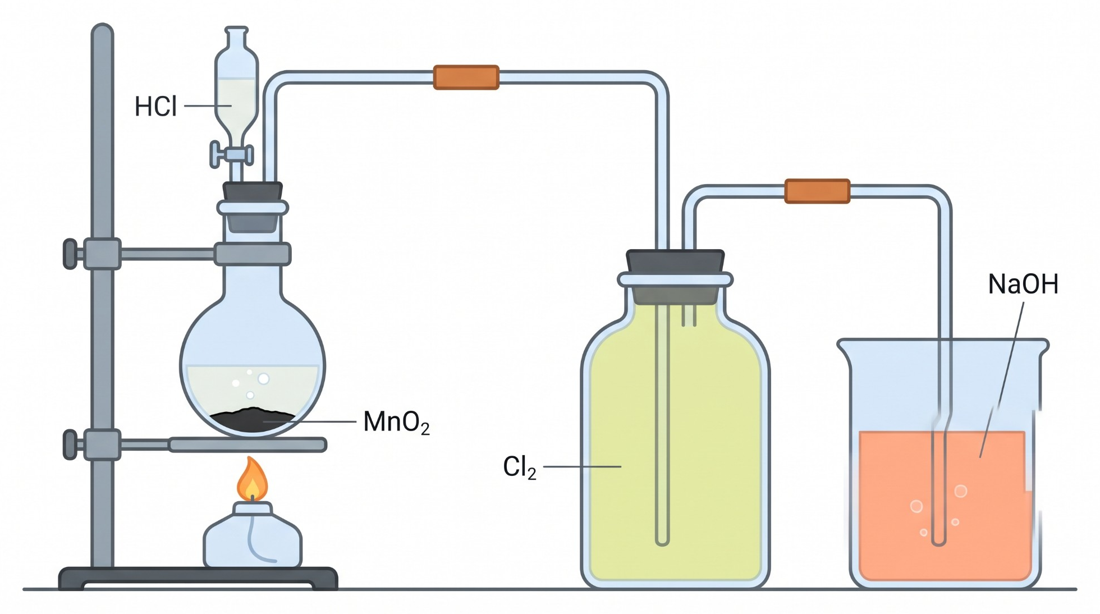
\includegraphics[width=0.86\linewidth]{rasmlar/darslik/d_xlor.png}\end{center}
\noindent A)~\textsl{MnO\textsubscript{2} va konsentrlangan HCl}\par
\noindent B)~\textsl{NH\textsubscript{4}Cl va Ca(OH)\textsubscript{2}}\par
\noindent C)~\textsl{Zn va HCl}\par
\noindent D)~\textsl{CaCO\textsubscript{3} va HCl}\par
\qsep
\noindent\qn{32.} Laboratoriyada vodorod sulfid olish uchun qaysi moddalar ishlatiladi?
\noindent A)~\textsl{CaC\textsubscript{2} + H\textsubscript{2}O}\par
\noindent B)~\textsl{FeS + HCl}\par
\noindent C)~\textsl{CH\textsubscript{3}COONa + NaOH (qizdirish)}\par
\noindent D)~\textsl{MnO\textsubscript{2} + HCl (kons.)   ---}\par
\qsep
\end{multicols}
\medskip
\noindent\setlength{\fboxsep}{0pt}\fbox{\begin{tabular}{p{0.74\linewidth}|p{0.2\linewidth}}
\parbox[t]{0.72\linewidth}{\vspace{3pt}\textbf{Topshiriqlar (33--35) va javob variant (A--F)larini o`zaro to`g`ri moslashtiring.} Qo`rg`oshin(II) nitratning 0,01 mol/l li eritmasidan 500 ml olinib, inert elektrodlar yordamida 5 A tok kuchi bilan 96 s elektroliz qilindi (eritma hajmi o`zgarmadi deb hisoblang). Elektrolizdan keyin eritmaga mo`l KI eritmasi qo`shildi.
\vspace{3pt}} & \parbox[t]{0.19\linewidth}{\vspace{3pt}A~\textsl{1}\\[3pt]
B~\textsl{0,78}\\[3pt]
C~\textsl{1,03}\\[3pt]
D~\textsl{2,3}\\[3pt]
E~\textsl{2}\\[3pt]
F~\textsl{0,52}}\\ \hline
\parbox[t]{0.72\linewidth}{\vspace{2pt}\textbf{33. Katodda ajralgan qo`rg`oshin massasini (g) toping.}\vspace{2pt}} & \\ \hline
\parbox[t]{0.72\linewidth}{\vspace{2pt}\textbf{34. Elektroliz tugagach eritmaning pH ini hisoblang.}\vspace{2pt}} & \\ \hline
\parbox[t]{0.72\linewidth}{\vspace{2pt}\textbf{35. KI qo`shilganda hosil bo`lgan cho`kma massasini (g) aniqlang.}\vspace{2pt}} & 
\end{tabular}}
\par\bigskip
\noindent\qn{36.} Zn + HNO\textsubscript{3} $\to$ Zn(NO\textsubscript{3})\textsubscript{2} + NH\textsubscript{4}NO\textsubscript{3} + H\textsubscript{2}O reaksiya tenglamasini tenglang va barcha koeffitsiyentlar \textbf{yig`indisini aniqlang.} Tajriba laboratoriyada, chinni idishda o`tkazildi.
\javob\qsep
\noindent\qn{37.} 61,25 g KClO\textsubscript{3} reaksiyaga kirishdi. Barcha reaksiyalar 2 atm bosimda olib borildi. Ajralgan O\textsubscript{2} \textbf{hajmini (l, n.sh.) hisoblang} (unum 90\%).
\javob\qsep
\noindent\qn{38.} Alyuminiy va mis dan iborat 9,1 g aralashma mo`l NaOH eritmasida eritildi. Reagent (NaOH) eritmasining massa ulushi 10\% va zichligi 1,05 g/ml; u mo`l miqdorda olingan. Ajralgan gazning \textbf{hajmini (l, n.sh.) aniqlang.}
\javob\qsep
\noindent\qn{39.} Vodorodga nisbatan zichligi 15 bo`lgan alkanning 30 g miqdorining 2/5 qismi yorug`likda xlor bilan monoxlorlandi, hosil bo`lgan xloralkan mo`l KOH ning suvli eritmasi bilan gidrolizlandi. Hosil bo`lgan spirtning \textbf{massasini (g) toping.}
\javob\qsep
\noindent\qn{40.} 44 g etilatsetat mo`l NaOH bilan qizdirilganda uning 1/2 qismi gidrolizlandi. Hosil bo`lgan spirt to`liq yondirildi. Qizdirish 60 daqiqa davom etdi. Yondirishda ajralgan CO\textsubscript{2} \textbf{hajmini (l, n.sh.) toping.}
\javob\qsep
\par\bigskip\begin{center}\textbf{\fontsize{13}{15}\selectfont YOZMA ISH}\end{center}
\noindent\qn{41.} \textbf{Topshiriqni bajarish jarayonida barcha reaksiya tenglamalarini yozing. Miqdoriy va arifmetik hisoblashlarni (unga asos bo`lgan usul yoki formulani ko`rsatgan holda) uzviy ketma-ketlikda bajaring.}\par\smallskip
63,2 g KMnO\textsubscript{4} qizdirilganda qisman parchalandi. Ajralgan kislorodning hajmi 27 \textdegree{}C va 83,14 kPa da 3 l ga teng bo`ldi (R = 8,314 J/(mol$\cdot$K)). Qattiq qoldiq mo`l konsentrlangan xlorid kislota bilan qizdirildi (K\textsubscript{2}MnO\textsubscript{4}, MnO\textsubscript{2} va parchalanmay qolgan KMnO\textsubscript{4} ning barchasi reaksiyaga kirishdi).\par
\noindent 1)\ Parchalanish va qattiq qoldiqning xlorid kislota bilan reaksiyalarini yozing va tenglashtiring (elektron balans).\par
\noindent 2)\ KMnO\textsubscript{4} ning necha foizi parchalanganini aniqlang.\par
\noindent 3)\ Qattiq qoldiq massasini (g) va undagi MnO\textsubscript{2} ning massa ulushini (\%) toping.\par
\noindent 4)\ Ajralgan xlorning umumiy hajmini (l, n.sh.) va sarflangan HCl miqdorini (mol) hisoblang.\par
\noindent 5)\ Reaksiyadan so`ng eritmadagi tuzlarning (KCl va MnCl\textsubscript{2}) umumiy massasini (g) toping.\par
\diqqat{Mazkur topshiriq kengaytirilgan javobni talab etib, uning yechilish usuli va shu usul asosidagi barcha hisoblash amallari javoblar varaqasida aks etishi lozim.}\qsep
\noindent\qn{42.} Organik moddalarning xossalarini bilgan holda reaksiya tenglamalarini tugallang va tenglashtiring. 3- va 5-reaksiyalarda hosil bo`lgan asosiy organik mahsulotlarni sistematik nomenklatura bo`yicha nomlang. Hosil bo`lgan organik moddalarning tuzilish formulalarini yozing.\par
\noindent 1)\ C\textsubscript{6}H\textsubscript{5}--OH + Br\textsubscript{2} (suvli eritma) $\to$\par
\noindent 2)\ CH\textsubscript{3}--COOH + Cl\textsubscript{2} (P, t) $\to$\par
\noindent 3)\ CH\textsubscript{3}--CH=CH--CH\textsubscript{3} + H\textsubscript{2}O (H\textsuperscript{+}) $\to$\par
\noindent 4)\ CH\textsubscript{3}--CH\textsubscript{2}--OH + CH\textsubscript{3}--COOH (H\textsubscript{2}SO\textsubscript{4}, t) $\rightleftarrows$\par
\noindent 5)\ CH\textsubscript{3}--CH\textsubscript{2}--OH (H\textsubscript{2}SO\textsubscript{4} kons., 170 \textdegree{}C) $\to$\par
\noindent 6)\ HCOOCH\textsubscript{3} + NaOH (t) $\to$\par
\noindent 7)\ CH\textsubscript{3}--CHCl--CH\textsubscript{3} + KOH (spirtli eritma, t) $\to$\par
\diqqat{Mazkur topshiriq kengaytirilgan javobni talab etib, uning yechilish usuli va shu usul asosidagi barcha hisoblash amallari javoblar varaqasida aks etishi lozim.}\qsep
\noindent\qn{43.} \textbf{Topshiriqni bajarish jarayonida barcha reaksiya tenglamalarini yozing. Miqdoriy va arifmetik hisoblashlarni (unga asos bo`lgan usul yoki formulani ko`rsatgan holda) uzviy ketma-ketlikda bajaring.}\par\smallskip
SO\textsubscript{2} va CO\textsubscript{2} dan iborat 6,72 l (n.sh.) gazlar aralashmasi avval mo`l bromli suvdan, so`ngra mo`l Ba(OH)\textsubscript{2} eritmasidan o`tkazildi. Bromli suvdan o`tgandan keyin SO\textsubscript{2} to`liq yutildi.\par
\noindent 1)\ Bromli suv bilan SO\textsubscript{2} reaksiyasi tenglamasini yozing. Hosil bo`lgan H\textsubscript{2}SO\textsubscript{4} massasini (g) toping. SO\textsubscript{2} hajmini (l, n.sh.) ham hisoblang.\par
\noindent 2)\ Mo`l BaCl\textsubscript{2} qo`shilganda bromli suvli eritmada hosil bo`lgan cho`kma massasini (g) aniqlang.\par
\noindent 3)\ Ba(OH)\textsubscript{2} eritmasida hosil bo`lgan cho`kma massasini (g) hisoblang.\par
\noindent 4)\ Dastlabki aralashmaning o`rtacha molyar massasini (g/mol) va havoga nisbatan zichligini toping.\par
\noindent 5)\ Bromli suvli eritmada hosil bo`lgan HBr massasini (g) hisoblang.\par
\diqqat{Mazkur topshiriq kengaytirilgan javobni talab etib, uning yechilish usuli va shu usul asosidagi barcha hisoblash amallari javoblar varaqasida aks etishi lozim.}\qsep
\newpage
\noindent\textbf{\fontsize{13}{15}\selectfont 20-variant}\hfill \textbf{Javoblar kaliti}\par\smallskip\hrule\smallskip
\textit{Faqat o`qituvchi uchun.}\par\medskip
\noindent\textbf{1--32-savollar}\par\smallskip
\noindent\begin{tabular}{|c|c|c|c|c|c|c|c|c|c|c|c|c|c|c|c|}\hline
\textbf{1} & \textbf{2} & \textbf{3} & \textbf{4} & \textbf{5} & \textbf{6} & \textbf{7} & \textbf{8} & \textbf{9} & \textbf{10} & \textbf{11} & \textbf{12} & \textbf{13} & \textbf{14} & \textbf{15} & \textbf{16}\\\hline
\textsl{C} & \textsl{B} & \textsl{C} & \textsl{C} & \textsl{D} & \textsl{B} & \textsl{C} & \textsl{C} & \textsl{A} & \textsl{D} & \textsl{A} & \textsl{A} & \textsl{C} & \textsl{B} & \textsl{B} & \textsl{D}\\\hline
\textbf{17} & \textbf{18} & \textbf{19} & \textbf{20} & \textbf{21} & \textbf{22} & \textbf{23} & \textbf{24} & \textbf{25} & \textbf{26} & \textbf{27} & \textbf{28} & \textbf{29} & \textbf{30} & \textbf{31} & \textbf{32}\\\hline
\textsl{D} & \textsl{A} & \textsl{A} & \textsl{C} & \textsl{D} & \textsl{B} & \textsl{D} & \textsl{A} & \textsl{B} & \textsl{A} & \textsl{D} & \textsl{C} & \textsl{B} & \textsl{D} & \textsl{A} & \textsl{B}\\\hline
\end{tabular}\par\medskip
\noindent\textbf{33--35-savollar}\par\smallskip
\noindent\begin{tabular}{|c|c|c|}\hline \textbf{No} & \textbf{Javob} & \textbf{Qiymat}\\\hline
33 & \textsl{F} & 0,52\\\hline
34 & \textsl{E} & 2\\\hline
35 & \textsl{D} & 2,3\\\hline
\end{tabular}\par\medskip
\noindent\textbf{36--40-savollar}\par\smallskip
\noindent\begin{tabular}{|c|c|}\hline \textbf{No} & \textbf{To`g`ri javob}\\\hline
36 & 22\\\hline
37 & 15,12\\\hline
38 & 3,36\\\hline
39 & 18,4\\\hline
40 & 11,2\\\hline
\end{tabular}\par\medskip
\noindent\textbf{41--43-topshiriqlar: javoblar}\par\smallskip
\noindent\textbf{41-topshiriq.}\par
\noindent 1) 2KMnO\textsubscript{4} $\to$ K\textsubscript{2}MnO\textsubscript{4} + MnO\textsubscript{2} + O\textsubscript{2}$\uparrow$; K\textsubscript{2}MnO\textsubscript{4} + 8HCl $\to$ 2KCl + MnCl\textsubscript{2} + 2Cl\textsubscript{2} + 4H\textsubscript{2}O; MnO\textsubscript{2} + 4HCl $\to$ MnCl\textsubscript{2} + Cl\textsubscript{2} + 2H\textsubscript{2}O; 2KMnO\textsubscript{4} + 16H\par
\noindent 2) 50\%\par
\noindent 3) 60 g; 14,5\%\par
\noindent 4) 17,92 l; 2,8 mol\par
\noindent 5) 80,2 g\par
\noindent\textbf{42-topshiriq.}\par
\noindent 1) C\textsubscript{6}H\textsubscript{5}--OH + 3Br\textsubscript{2} $\to$ C\textsubscript{6}H\textsubscript{2}Br\textsubscript{3}--OH$\downarrow$ + 3HBr\par
\noindent 2) CH\textsubscript{3}--COOH + Cl\textsubscript{2} $\to$ CH\textsubscript{2}Cl--COOH + HCl\par
\noindent 3) CH\textsubscript{3}--CH=CH--CH\textsubscript{3} + H\textsubscript{2}O $\to$ CH\textsubscript{3}--CH(OH)--CH\textsubscript{2}--CH\textsubscript{3} --- nomi: \textbf{butanol-2}\par
\noindent 4) CH\textsubscript{3}--CH\textsubscript{2}--OH + CH\textsubscript{3}--COOH $\rightleftarrows$ CH\textsubscript{3}--COO--CH\textsubscript{2}--CH\textsubscript{3} + H\textsubscript{2}O\par
\noindent 5) CH\textsubscript{3}--CH\textsubscript{2}--OH $\to$ CH\textsubscript{2}=CH\textsubscript{2} + H\textsubscript{2}O --- nomi: \textbf{etilen}\par
\noindent 6) HCOOCH\textsubscript{3} + NaOH $\to$ HCOONa + CH\textsubscript{3}OH\par
\noindent 7) CH\textsubscript{3}--CHCl--CH\textsubscript{3} + KOH $\to$ CH\textsubscript{3}--CH=CH\textsubscript{2} + KCl + H\textsubscript{2}O\par
\noindent\textbf{43-topshiriq.}\par
\noindent 1) 9,8 g; 2,24 l\par
\noindent 2) 23,3 g\par
\noindent 3) 39,4 g\par
\noindent 4) 50,67 g/mol; 1,75\par
\noindent 5) 16,2 g\par
\par\bigskip\noindent\textbf{Mavzular taqsimoti}\par\smallskip
{\small\noindent\begin{longtable}{|c|p{7.2cm}|p{5.4cm}|c|}\hline \textbf{No} & \textbf{Mavzu} & \textbf{Tekshiriladigan ko`nikma} & \textbf{Ball}\\\hline
1 & 9-sinf; 11-sinf (tuzlar gidrolizi; Le-Shatelye) & Bilim va tushunish & 1\\\hline
2 & 7-sinf (valentlik) & Bilim va tushunish & 1\\\hline
3 & 8-sinf (kimyoviy bog`lanish turlari, jadval) & Jadval tahlili & 1\\\hline
4 & Tirkashev I bob; 8-sinf (elektron konfiguratsiya) & Bilim va tushunish & 1\\\hline
5 & 8-sinf (davriy qonun, jadval) & Rasm bo`yicha tahlil & 1\\\hline
6 & 11-sinf 8-bob; Tirkashev \textit{V} bob (elektroliz) & Bilim va tushunish & 1\\\hline
7 & 11-sinf (Mendeleyev--Klapeyron) & Hisoblash va masala yechish & 1\\\hline
8 & 9-sinf; 11-sinf (tuzlar gidrolizi; Le-Shatelye) & Bilim va tushunish & 1\\\hline
9 & 7-sinf (Avogadro) & Hisoblash va masala yechish & 1\\\hline
10 & Tirkashev III bob (eruvchanlik, grafik) & Grafik tahlili & 1\\\hline
11 & Tirkashev III bob (eritmalar, jadval) & Jadval tahlili & 1\\\hline
12 & 8-9-sinf (gaz aralashmalari; Avogadro qonuni) & Hisoblash va masala yechish & 1\\\hline
13 & Tirkashev VI bob (muvozanat, jadval) & Jadval tahlili & 1\\\hline
14 & 9-sinf (ishqoriy metallar); Tashev & Bilim va tushunish & 1\\\hline
15 & 9-sinf; Tashev (Fe, Cu, Zn, Cr) & Bilim va tushunish & 1\\\hline
16 & 8-sinf; 9-sinf; Tashev (oksidlar sinflari) & Bilim va tushunish & 1\\\hline
17 & 9-sinf (Al, Mg, Ca) & Hisoblash va masala yechish & 1\\\hline
18 & 8-9-sinf (karbonatlar; kislotalar bilan reaksiya) & Hisoblash va masala yechish & 1\\\hline
19 & 9-sinf (metallarning kuchlanish qatori; plastinka massasi o`zgarishi) & Hisoblash va masala yechish & 1\\\hline
20 & 10-sinf (nomenklatura \S{}6, \S{}11, \S{}20, \S{}24--26) & Bilim va tushunish & 1\\\hline
21 & 10-sinf (mavzuga oid paragraflar); Abdusamatov & Bilim va tushunish & 1\\\hline
22 & 10-sinf (mavzuga oid paragraflar); Abdusamatov & Bilim va tushunish & 1\\\hline
23 & 10-sinf (alkan va alkenlarning galogenli hosilalari) & Hisoblash va masala yechish & 1\\\hline
24 & 10-sinf (aminlar va anilin xossalari) & Hisoblash va masala yechish & 1\\\hline
25 & 10-sinf (alkinlar, alkenlar, spirtlar) & Hisoblash va masala yechish & 1\\\hline
26 & 10-sinf (polimerlar; vinilxlorid olinishi) & Hisoblash va masala yechish & 1\\\hline
27 & 10-sinf (karbon kislotalar; chumoli kislotaning o`ziga xosligi) & Hisoblash va masala yechish & 1\\\hline
28 & 10-sinf (spirtlar, alkenlar, ko`p atomli spirtlar) & Hisoblash va masala yechish & 1\\\hline
29 & 10-sinf (Lebedev usuli; sintetik kauchuk) & Hisoblash va masala yechish & 1\\\hline
30 & 10-sinf (spirt, aldegid, fenol sifat reaksiyalari) & Bilim va tushunish & 1\\\hline
31 & 8-sinf (xlor olinishi, 15-rasm) & Rasm bo`yicha tahlil & 1\\\hline
32 & 9--10-sinf (laboratoriya usullari bilan gaz olish) & Bilim va tushunish & 1\\\hline
33--35 & Aralash masala (moslashtirish) & Ko`p bosqichli hisob & 3\\\hline
36--40 & Qisqa javobli masalalar & Hisoblash & 5\\\hline
41--43 & Yozma ish & Usul va hisob (M, A) & 75\\\hline
\end{longtable}}
\end{document}
